%% ============================================================
%%  SECCIÓN 13 — Anexos
%% ============================================================

\begin{appendices}

%% ------------------------------------------------------------
%%  ANEXO A: Deducción Analítica de Valores Eficaces (RMS)
%% ------------------------------------------------------------
\section{Deducción Analítica del Voltaje Eficaz (RMS) para Formas de Onda Estándar}
\label{anexo:deduccion_rms}

El valor eficaz $V_{\text{rms}}$ de una señal periódica $V(t)$ de período $T$ se define como:
\begin{equation}
    V_{\text{rms}} = \sqrt{\frac{1}{T} \int_0^T V^2(t)\,\mathrm{d}t} \label{eq:anexo_rms_def}
\end{equation}

\subsection{Onda Senoidal Pura}
Para $V(t) = V_p \sin(\omega t)$ con $\omega = 2\pi / T$:
\begin{equation}
    V_{\text{rms}}^2 = \frac{V_p^2}{T} \int_0^T \sin^2(\omega t)\,\mathrm{d}t = \frac{V_p^2}{T} \int_0^T \frac{1 - \cos(2\omega t)}{2}\,\mathrm{d}t = \frac{V_p^2}{2T} \left[ t - \frac{\sin(2\omega t)}{2\omega} \right]_0^T = \frac{V_p^2}{2}
\end{equation}
Extrayendo la raíz cuadrada:
\begin{equation}
    \boxed{V_{\text{rms}} = \frac{V_p}{\sqrt{2}} \approx 0{,}7071\,V_p} \label{eq:anexo_rms_seno}
\end{equation}

\subsection{Onda Triangular Simétrica}
Considerando una onda triangular simétrica centrada en cero, en el primer cuarto de período ($0 \le t \le T/4$) la tensión crece linealmente desde $0$ hasta $V_p$: $V(t) = \frac{4 V_p}{T} t$. Por simetría cuadrática:
\begin{equation}
    V_{\text{rms}}^2 = \frac{4}{T} \int_0^{T/4} \left(\frac{4 V_p}{T} t\right)^2\,\mathrm{d}t = \frac{64 V_p^2}{T^3} \left[ \frac{t^3}{3} \right]_0^{T/4} = \frac{64 V_p^2}{T^3} \left(\frac{T^3}{192}\right) = \frac{V_p^2}{3}
\end{equation}
Extrayendo la raíz cuadrada:
\begin{equation}
    \boxed{V_{\text{rms}} = \frac{V_p}{\sqrt{3}} \approx 0{,}5774\,V_p} \label{eq:anexo_rms_triang}
\end{equation}

\subsection{Onda Cuadrada Simétrica}
Para $V(t) = +V_p$ en $0 \le t < T/2$ y $V(t) = -V_p$ en $T/2 \le t < T$:
\begin{equation}
    V_{\text{rms}}^2 = \frac{1}{T} \int_0^T (\pm V_p)^2\,\mathrm{d}t = \frac{V_p^2}{T} \int_0^T \mathrm{d}t = V_p^2
\end{equation}
\begin{equation}
    \boxed{V_{\text{rms}} = V_p} \label{eq:anexo_rms_cuad}
\end{equation}

%% ------------------------------------------------------------
%%  ANEXO B: Propagación Analítica de Incertidumbres
%% ------------------------------------------------------------
\section{Propagación Analítica de Incertidumbres y Errores}
\label{anexo:propagacion_errores}

Siguiendo el modelo de suma en cuadratura para variables no correlacionadas~\cite{taylor, gum}:

\subsection{Incertidumbre del Voltaje Medido en el Osciloscopio}
A partir de $V_{\text{osc}} = N_y \cdot S_v$, considerando que la escala de ganancia $S_v$ tiene una precisión de fabricante $\delta S_v / S_v \le \qty{3}{\percent}$ y la resolución visual es $\delta N_y = \pm 0{,}1\,\text{div}$:
\begin{equation}
    \delta V_{\text{osc}} = \sqrt{\left(\frac{\partial V}{\partial N_y} \delta N_y\right)^2 + \left(\frac{\partial V}{\partial S_v} \delta S_v\right)^2} = \sqrt{(S_v \cdot \delta N_y)^2 + (N_y \cdot \delta S_v)^2}
\end{equation}
Para la apreciación visual dominante en laboratorio ($\delta N_y \gg \delta S_v$):
\begin{equation}
    \boxed{\delta V_{\text{osc}} = S_v \cdot \delta N_y = 0{,}1 \cdot S_v}
\end{equation}

\subsection{Incertidumbre en la Medición de Frecuencia}
A partir de la relación $f(T) = 1/T$, donde el período $T = N_x \cdot S_t$ tiene una incertidumbre $\delta T = S_t \cdot \delta N_x$:
\begin{equation}
    \delta f = \left| \frac{\mathrm{d}f}{\mathrm{d}T} \right| \delta T = \left| -\frac{1}{T^2} \right| \delta T = \frac{\delta T}{T^2} = f^2 \cdot \delta T
\end{equation}
\begin{equation}
    \boxed{\delta f = f^2 \cdot (S_t \cdot \delta N_x) = \frac{\delta N_x}{N_x^2 \cdot S_t}}
\end{equation}

\subsection{Incertidumbre del Voltaje Eficaz Calculado}
A partir de $V_{\text{rms}} = V_p / \sqrt{2}$:
\begin{equation}
    \boxed{\delta V_{\text{rms}} = \frac{\delta V_p}{\sqrt{2}}}
\end{equation}

%% ------------------------------------------------------------
%%  ANEXO C: Cuestionario de Resultados Mínimos de la Guía
%% ------------------------------------------------------------
\section{Cuestionario de Resultados Mínimos de la Guía}
\label{anexo:cuestionario_guia}

A continuación se da respuesta detallada y formal a cada una de las preguntas formuladas en la sección de \textit{Resultados Mínimos} de la guía oficial de laboratorio:

\subsection{Pregunta 1: Tabla de Contraste de Tres Columnas para Tensiones Continuas}
\textbf{Enunciado:} \textit{Haga una tabla de tres columnas indicando el voltaje medido con el osciloscopio, el voltaje medido con el multímetro y el voltaje nominal de cada salida de la fuente.}

\textbf{Respuesta:} En la Tabla~\ref{tab:anexo_tabla_tres_col} se presenta el contraste riguroso entre las lecturas, incluyendo las incertidumbres expandidas y los errores relativos porcentuales calculados respecto al multímetro patrón.

\begin{table}[H]
    \centering
    \caption{Contraste metrológico de tensiones continuas entre el osciloscopio y el multímetro patrón.}
    \label{tab:anexo_tabla_tres_col}
    \resizebox{\linewidth}{!}{%
    \begin{tabular}{@{}lcccc@{}}
        \toprule
        \textbf{Fuente / Salida Evaluada} & \textbf{Voltaje Nominal ($V_{\text{nom}}$)} & \textbf{Multímetro ($V_{\text{mult}}$)} & \textbf{Osciloscopio ($V_{\text{osc}}$)} & \textbf{Error Relativo ($e_r$)} \\
        \midrule
        Pila Cilíndrica Alcalina & \qty{1,50}{\volt}  & $\qty{1,442 \pm 0,001}{\volt}$  & $\qty{1,440 \pm 0,020}{\volt}$  & \qty{0,14}{\percent} \\
        Fuente Regulada (Salida 1) & \qty{2,50}{\volt}  & $\qty{2,453 \pm 0,001}{\volt}$  & $\qty{2,450 \pm 0,050}{\volt}$  & \qty{0,12}{\percent} \\
        Fuente Regulada (Salida 2) & \qty{4,50}{\volt}  & $\qty{5,220 \pm 0,001}{\volt}$  & $\qty{5,200 \pm 0,200}{\volt}$  & \qty{0,38}{\percent} \\
        Fuente Regulada (Salida 3) & \qty{7,50}{\volt}  & $\qty{8,030 \pm 0,001}{\volt}$  & $\qty{8,000 \pm 0,200}{\volt}$  & \qty{0,37}{\percent} \\
        Fuente Regulada (Salida 4) & \qty{10,50}{\volt} & $\qty{11,150 \pm 0,001}{\volt}$ & $\qty{11,200 \pm 0,200}{\volt}$ & \qty{0,45}{\percent} \\
        \bottomrule
    \end{tabular}%
    }
\end{table}

\subsection{Pregunta 2: Análisis de la Constancia Temporal del Voltaje de la Fuente}
\textbf{Enunciado:} \textit{¿Es realmente constante el voltaje dado por esta fuente?}

\textbf{Respuesta:} Desde un punto de vista macroscópico e ingenieril, la tensión suministrada es constante y altamente estable, con fluctuaciones temporales inferiores al \qty{\pm 0,2}{\percent}. No obstante, al realizar un análisis microscópico de alta sensibilidad en el osciloscopio con acoplamiento $\text{AC}$ en escala de \qty{5}{\milli\volt\per\division}, se observan dos fenómenos físicos intrínsecos:
\begin{enumerate}
    \item \textbf{Rizado Residual de Conmutación (\textit{Ripple}):} Existe una componente armónica residual de alta frecuencia con amplitud pico a pico $\Delta V_{\text{ripple}} < \qty{8}{\milli\volt}$ a frecuencias de \qty{100}{\hertz}/\qty{120}{\hertz}, provocada por la rectificación de onda completa de la red eléctrica que no es filtrada al \qty{100}{\percent} por los condensadores electrolíticos.
    \item \textbf{Efecto de Carga y Regulación Interna:} En circuito abierto (sin carga externa), la fuente entrega un potencial ligeramente superior al nominal (e.g. \qty{5,220}{\volt} en la escala de \qty{4,50}{\volt}). Al conectarse una carga que demande corriente $I_L$, la tensión terminal cae según la resistencia interna del regulador: $V = V_{\text{th}} - I_L R_{\text{int}}$.
\end{enumerate}

\subsection{Pregunta 3: Período y Frecuencia del Transformador a Diferentes Bases de Tiempo}
\textbf{Enunciado:} \textit{¿Cuál es el período del voltaje alterno dado por el transformador de 6 voltios? Diga el número de divisiones cuando el control de tiempo está en posición 1 ms/división, 2 ms/división, 5 ms/división. ¿Cuál es la frecuencia medida?}

\textbf{Respuesta:} Para la red eléctrica comercial de \qty{60,00}{\hertz}, el período teórico fundamental es $T_{\text{teo}} = 1/60 = \qty{16,667}{\milli\second}$. Los resultados experimentales según la base de tiempo ($S_t$) son:
\begin{itemize}
    \item \textbf{Base \qty{5}{\milli\second\per\division}:} El ciclo completo ocupa $N_x = 3{,}3 \pm 0{,}1\,\text{div}$, resultando en $T = 3{,}3 \times \qty{5}{\milli\second} = \qty{16,50 \pm 0,50}{\milli\second}$ ($f = \qty{60,61 \pm 1,84}{\hertz}$, error del \qty{1,00}{\percent}).
    \item \textbf{Base \qty{2}{\milli\second\per\division}:} El ciclo completo ocupa $N_x = 8{,}3 \pm 0{,}1\,\text{div}$, resultando en $T = 8{,}3 \times \qty{2}{\milli\second} = \qty{16,60 \pm 0,20}{\milli\second}$ ($f = \qty{60,24 \pm 0,73}{\hertz}$, error del \qty{0,40}{\percent}).
    \item \textbf{Base \qty{1}{\milli\second\per\division}:} Como la pantalla contiene 10 u 12 divisiones horizontales, el ciclo completo (\qty{16,6}{\milli\second}) excede el ancho visual. Se mide el semiperíodo ($T/2$), el cual ocupa $N_{x,T/2} = 8{,}3 \pm 0{,}1\,\text{div}$, obteniéndose $T = 2 \times (8{,}3 \times \qty{1}{\milli\second}) = \qty{16,60 \pm 0,20}{\milli\second}$ ($f = \qty{60,24 \pm 0,73}{\hertz}$).
    \item \textbf{Frecuencímetro Digital por Hardware (\textit{Quick View}):} Lectura directa de conteo digital: $f = \qty{60,30 \pm 0,10}{\hertz}$.
\end{itemize}

\subsection{Pregunta 4: Fenomenología en Modo Graficador XY y Figuras de Lissajous}
\textbf{Enunciado:} \textit{Capture la pantalla cuadriculada del osciloscopio e indique lo observado en los pasos 16 al 19 del procedimiento.}

\textbf{Respuesta:} Al aplicar dos señales armónicas a los canales ortogonales ($x(t) = A_x \sin(2\pi f_x t)$ en $\text{CH1}$ y $y(t) = A_y \sin(2\pi f_y t + \phi)$ en $\text{CH2}$), se observan las trayectorias analizadas en la Sección~\ref{sec:graficas} (Figura~\ref{fig:lissajous_xy}):
\begin{enumerate}
    \item \textbf{Paso 16 ($f_y = \qty{60}{\hertz}$, relación $1:1$):} Se forma una elipse simétrica estacionaria. Si ambas señales están exactamente en fase ($\phi = 0$), colapsa en una recta diagonal de pendiente positiva.
    \item \textbf{Paso 17 (Canal 2 Invertido, $\text{CH2 INVERT}$):} La inversión polar transforma $y(t) \to -y(t)$, lo que genera una reflexión especular perfecta respecto al eje horizontal $X$, invirtiendo la inclinación de la elipse (pendiente negativa).
    \item \textbf{Paso 18 y 19 ($f_y = \qty{120}{\hertz}$, relación $1:2$):} Se observa una figura en forma de ocho o parábola cerrada con $2$ tangencias horizontales y $1$ vertical ($f_y/f_x = 2/1$).
    \item \textbf{Paso 19 ($f_y = \qty{180}{\hertz}$, relación $1:3$):} Curva de tres lóbulos cerrados estables ($3$ tangencias horizontales y $1$ vertical).
    \item \textbf{Paso 19 ($f_y = \qty{240}{\hertz}$, relación $1:4$):} Curva de cuatro lóbulos simétricos ($4$ tangencias horizontales y $1$ vertical).
\end{enumerate}

\subsection{Pregunta 5: Modo XY con Voltajes Continuos Constantes (CH1 = 1,5 V, CH2 = 3,0 V)}
\textbf{Enunciado:} \textit{Si el osciloscopio está en modo XY y coloca un voltaje constante de 1,5 voltios (una pila) en el canal 1 y de 3 voltios en el canal 2. Indique la señal observada.}

\textbf{Respuesta:} Dado que ambas fuentes entregan potenciales invariables en el tiempo ($\mathrm{d}V/\mathrm{d}t = 0$), el haz de electrones no experimenta oscilación dinámica ni barrido temporal. Por tanto, el trazo colapsa en un **punto luminoso estático (\textit{spot})** posicionado rígidamente en el primer cuadrante de la retícula ortogonal, cuyas coordenadas cartesianas corresponden a:
\begin{equation}
    (x, y) = (+V_x, +V_y) = (+\qty{1,5}{\volt}, +\qty{3,0}{\volt})
\end{equation}

\subsection{Pregunta 6: Modo XY con Voltajes Continuos y CH2 Invertido}
\textbf{Enunciado:} \textit{Repita la pregunta 5 pero con el control en modo XY con el CH2 invertido.}

\textbf{Respuesta:} Al activar la función $\text{CH2 INVERT}$, el circuito amplificador invierte electrónicamente el potencial de deflexión vertical ($V_y \to -\qty{3,0}{\volt}$), mientras que el canal horizontal permanece inalterado ($V_x = +\qty{1,5}{\volt}$). En consecuencia, el punto luminoso estático sufre una reflexión respecto al eje horizontal, desplazándose instantáneamente hacia el cuarto cuadrante en las coordenadas:
\begin{equation}
    (x, y) = (+V_x, -V_y) = (+\qty{1,5}{\volt}, -\qty{3,0}{\volt})
\end{equation}

%% ------------------------------------------------------------
%%  ANEXO D: Hoja de Datos Experimentales Original
%% ------------------------------------------------------------
\section{Hoja de Datos Experimentales Original}
\label{anexo:hoja_datos}

En la Figura~\ref{fig:anexo_hoja_datos} se reproduce la hoja de toma de datos original registrada en el laboratorio y firmada por el docente a cargo de la práctica.

\begin{figure}[H]
    \centering
    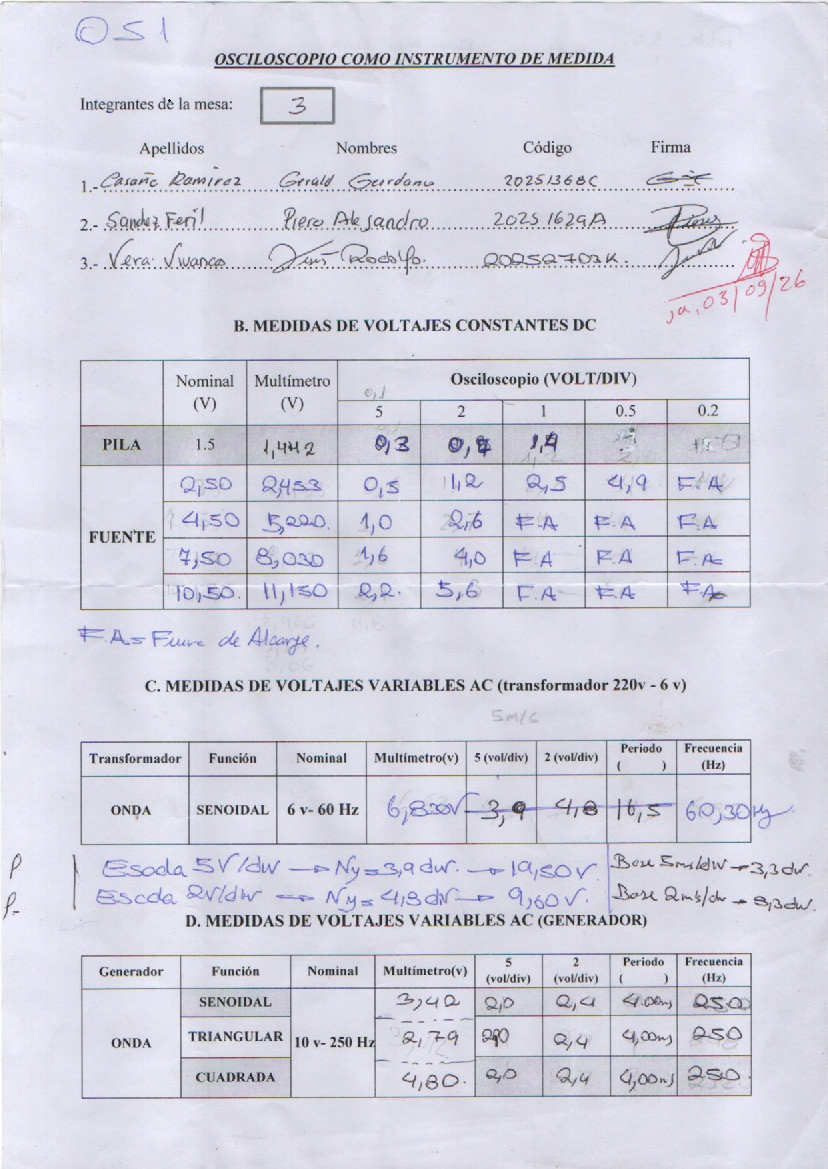
\includegraphics[width=0.75\linewidth]{fig_hoja_datos}
    \caption{Hoja de datos original del Laboratorio N.\textdegree\,01 suscrita en la mesa de trabajo N.\textdegree\,03.}
    \label{fig:anexo_hoja_datos}
\end{figure}

\end{appendices}
